\documentclass{article}
\usepackage{tikz}
\usetikzlibrary{calc}
\usepackage{xcolor}
\definecolor{papercolor}{HTML}{313131}
%\definecolor{linecolor}{HTML}{}
\begin{document}
\pagestyle{empty}
\pagecolor{papercolor}
\begin{tikzpicture}[remember picture,overlay]
% \foreach \i in {1,2,...,27}{
% \draw[line width = 0.2mm, blue] ($(current page.north west)+(0,-\i)$) -- ($(current page.north east)+(0,-\i)$);
%}
\draw[step=0.55cm,black,line width=0.1mm] (current page.south west) grid (current page.north east);
\draw[line width = 0.7mm, cyan](current page.north) -- (current page.south);
\end{tikzpicture}
\end{document}
 
